\documentclass{beamer}



\usepackage[english]{babel}
\usepackage{algorithm}
\usepackage{algpseudocode}

\usepackage[utf8]{inputenc}

\usepackage[english]{babel}
\usepackage{verbatim}
\usepackage{graphicx}
\usepackage{subcaption}
\usepackage{mwe}
\usepackage{amsmath}
\usepackage{bm}
\usepackage{tikz}
\usepackage{verbatim}
\usepackage{textcomp}
\usetikzlibrary{fit, positioning, shapes,arrows}
\usepackage{multirow}
\usepackage{multicol} % Required for multiple columns
\usepackage{algorithm}
\usepackage{algpseudocode}
\usepackage[utf8]{inputenc}
\usepackage[english]{babel}
\usepackage{appendixnumberbeamer}
\DeclareMathOperator{\EX}{\mathbb{E}}% expected value
\usepackage{graphicx}

\usepackage{hyperref}       % hyperlinks
\usepackage{url}            % simple URL typesetting
\usepackage{booktabs}       % professional-quality tables
\usepackage{amsfonts}       % blackboard math symbols
\usepackage{nicefrac}       % compact symbols for 1/2, etc.
\usepackage{microtype}      % microtypography
\usepackage{algorithm}
\usepackage{bm}


\tikzset{three sided/.style={
        draw=none,
        append after command={
            [shorten <= -0.5\pgflinewidth]
            ([shift={(-1.5\pgflinewidth,-0.5\pgflinewidth)}]\tikzlastnode.north east)
        edge([shift={( 0.5\pgflinewidth,-0.5\pgflinewidth)}]\tikzlastnode.north west) 
            ([shift={( 0.5\pgflinewidth,-0.5\pgflinewidth)}]\tikzlastnode.north west)
        edge([shift={( 0.5\pgflinewidth,+0.5\pgflinewidth)}]\tikzlastnode.south west)            
            ([shift={( 0.5\pgflinewidth,+0.5\pgflinewidth)}]\tikzlastnode.south west)
        edge([shift={(-1.0\pgflinewidth,+0.5\pgflinewidth)}]\tikzlastnode.south east)
        }
    }
}

\makeatletter
\DeclareRobustCommand{\rchi}{{\mathpalette\irchi\relax}}
\newcommand{\irchi}[2]{\raisebox{\depth}{$#1\chi$}} 

\newcommand*\bigcdot{\mathpalette\bigcdot@{.5}}
\newcommand*\bigcdot@[2]{\mathbin{\vcenter{\hbox{\scalebox{#2}{$\m@th#1\bullet$}}}}}
\makeatother



% to compile a camera-ready version, add the [final] option, e.g.:
% \usepackage[final]{nips_2016}

\usepackage{nicefrac}       % compact symbols for 1/2, etc.
\usepackage{microtype}      % microtypography
\setbeamerfont{caption}{series=\normalfont,size=\fontsize{6}{6}} 
\usepackage{breakcites}
\usepackage[tableposition=top]{caption}

\usepackage{ragged2e}
\usepackage{etoolbox}
\usepackage{lipsum}


\apptocmd{\frame}{}{\justifying}{} % Allow optional arguments after frame.

\colorlet{Mycolor1}{green!10!orange!90!}
\definecolor{foreground}{RGB}{255,255,255}
\definecolor{background}{RGB}{30,30,30}
\definecolor{title}{RGB}{107,174,214}
\definecolor{gray}{RGB}{155,155,155}
\definecolor{subtitle}{RGB}{102,255,204}
\definecolor{hilight}{RGB}{102,255,204}
\definecolor{vhilight}{RGB}{255,111,207}
\definecolor{footline}{RGB}{255,255,255}

\setbeamercolor{titlelike}{fg=title}
\setbeamercolor{subtitle}{fg=subtitle}
\setbeamercolor{institute}{fg=gray}
\setbeamercolor{normal text}{fg=foreground,bg=background}

\usepackage{lipsum}

\defbeamertemplate{headline}{page number}{%
	\vskip1pt%
	\setbeamertemplate{footline}[page number]%
	\usebeamertemplate{footline}%
}
\setbeamertemplate{headline}[page number]
\setbeamercolor{page number in head/foot}{fg=white}



\usepackage[absolute,overlay]{textpos}

\mode<presentation>
{
  \usetheme{default}      % or try Darmstadt, Madrid, Warsaw, ...
  \usecolortheme{default} % or try albatross, beaver, crane, ...
  \usefonttheme{default}  % or try serif, structurebold, ...
  \setbeamertemplate{navigation symbols}{}
  \setbeamertemplate{caption}[numbered]
} 
\usepackage{acronym}

%%Theo's stuff
\newcommand{\theo}[1]{{\color{blue}Theo: [#1]}}
\newcommand{\edwin}[1]{{\color{green}Edwin: [#1]}}
\newcommand{\virginia}[1]{{\color{red}Virginia: [#1]}}

% abbreviations
\newcommand{\etal}{et al.\xspace}
\newcommand{\ie}{i.e.\xspace}
\newcommand{\eg}{e.g.\xspace}
\newcommand{\Ie}{I.e.\xspace}
\newcommand{\eq}{Eq.\xspace}
\newcommand{\eqs}{Eqs.\xspace}
\newcommand{\fig}{Fig.\xspace}
\newcommand{\secref}[1]{\S \ref{#1}}
\newcommand{\iid}{i.i.d.~\xspace}
\newcommand{\dgp}{DGP\xspace}
\newcommand{\tbl}{Tab.\xspace}


% Acronyms
\newcommand{\supplement}{supplement}
\newcommand{\acro}[1]{\textsc{#1}\xspace}
\newcommand{\lgcp}{\acro{lgcp}}
\newcommand{\icm}{\acro{icm}}
\newcommand{\lgcpn}{\acro{lgcpn}}
\newcommand{\lgcpnnormal}{\acro{lgcpn-n}}
\newcommand{\lgcpngp}{\acro{lgcpn-gp}}
\newcommand{\mlgcp}{\acro{mlgcp}}
\newcommand{\pool}{\acro{pooling}}
\newcommand{\lgcpc}{\acro{lgcp-c}}
\newcommand{\lgcpnc}{\acro{lgcpn-c}}
\newcommand{\gptext}{\acro{gp}}
\newcommand{\mtl}{\acro{mtl}}
\newcommand{\stl}{\acro{stl}}
\newcommand{\mcmc}{\acro{mcmc}}
\newcommand{\mala}{\acro{mala}}
\newcommand{\inla}{\acro{inla}}
\newcommand{\lcm}{\acro{lcm}}
\newcommand{\rbf}{\acro{rbf}}
\newcommand{\btb}{\acro{btb}}
\newcommand{\gt}{\acro{gt}}
\newcommand{\mv}{\acro{mv}}
\newcommand{\nypd}{\acro{nypd}}
\newcommand{\nlpl}{\acro{nlpl}}
\newcommand{\rmse}{\acro{rmse}}
\newcommand{\crime}{\acro{crime}}
\newcommand{\cpu}{\acro{cpu}}
\newcommand{\gb}{\acro{gb}}
\newcommand{\ram}{\acro{ram}}


% Matrices and vectors 
\newcommand{\mat}[1]{\mathbf{#1}}
\renewcommand{\vec}[1]{ \mathbf{#1} } % math bold
\newcommand{\vecS}[1]{\boldsymbol{ #1 }  } % this for boldsymbols
\newcommand{\vecentry}[2]{{\mathrm #1_{#2}}}
\newcommand{\matentry}[3]{{\mathrm #1_{#2,#3}}}
\newcommand{\matcol}[2]{\mat{#1}_{\cdot,#2}}
\newcommand{\matrow}[2]{\mat{#1}_{#2,\cdot}}

% GP things
\newcommand{\gp}{\mathcal{GP}}
\newcommand{\kernel}{\kappa}
\newcommand{\meanfunc}[1]{m(#1)}
\newcommand{\covfunc}[3]{\kernel(#1,#2; #3)}
\newcommand{\hyperparam}{\vectheta}

% Specific variables
\newcommand{\dataset}{\mathcal{D}}
\newcommand{\x}{\vec{x}}
\newcommand{\xn}{\x_n}
\newcommand{\xstar}{\x_\star}
\newcommand{\xprime}{\x^{\prime}}
\newcommand{\vectheta}{\vecS{\theta}}
\newcommand{\y}{\vec{y}}
\newcommand{\ystar}{\y_\star}
\newcommand{\yn}{\vec{y}_n}
\newcommand{\f}{\mat{F}}
\newcommand{\fstar}{\f_\star}
%\newcommand{\u}{\vec{u}}
\newcommand{\fq}{\f_{\bullet q}}
\newcommand{\fn}{\f_{n \bullet}}
\newcommand{\samplefn}[1]{\fn^{(#1)}}
\newcommand{\W}{\mat{W}}
\renewcommand{\wp}{\W_{p \bullet}}
\newcommand{\varw}{\sigma^2} % variance of W for independent prior
\newcommand{\wq}{\W_{\bullet q}}
\newcommand{\samplewp}[1]{\wp^{(#1)}}
\newcommand{\Y}{\mat{Y}}
\newcommand{\lambdan}{\vec{\lambda}_{n \bullet}}
\renewcommand{\u}{\mat{U}}
\newcommand{\uq}{\u_{\bullet q}}
\newcommand{\z}{\vec{z}}
\newcommand{\Z}{\mat{Z}}
\newcommand{\Zq}{\Z_q}
\newcommand{\zprime}{\z^{\prime}}
\newcommand{\meanfu}{\tilde{\vecS{\mu}}}  % conditonal prior mean
\newcommand{\covfu}{\widetilde{\vecS{\mat{K}}}}  % conditonal prior covariance
\newcommand{\meanfuq}{\tilde{\vecS{\mu}}_q}  % conditonal prior mean
\newcommand{\covfuq}{\widetilde{\vecS{\mat{K}}}_q}  % conditonal prior covariance
\newcommand{\likeparam}{\phi}

% Covariance matricces
\newcommand{\Kq}{\mat{K}_{xx}^q}
\newcommand{\covwq}{\vecS{\mat{K}}_{w}^q}
\newcommand{\Kzzq}{\mat{K}_{zz}^q}
\newcommand{\Kxzq}{\mat{K}_{xz}^q}
\newcommand{\Kzxq}{\mat{K}_{zx}^q}
\newcommand{\Kzzqinv}{(\mat{K}_{zz}^q)^{-1}}


% Distributions
\newcommand{\poisson}{\text{Poisson}}
\newcommand{\normal}{\mathcal{N}}

% statistics / algebra / computation
\newcommand{\kl}[2]{\mathrm{KL}(#1 \lVert #2)}
\newcommand{\expectation}[2]{ \mathbb{E}_{#1}{\left[#2\right]} }
\renewcommand{\det}[1]{\left\lvert#1\right\rvert}
\newcommand{\trace}{\mbox{ \rm tr }}
\newcommand{\bigO}{\mathcal{O}}

% variational stuff
\newcommand{\varparam}{\vecS{\nu}}
\newcommand{\varmeanuq}{\vec{m}_q}
\newcommand{\varmeanfqn}{\mu_q}
\newcommand{\varmeanfq}{\pmb{\mu}_q}
\newcommand{\varcovuq}{\mat{S}_q}
\newcommand{\varmeanwq}{\vecS{\omega}_q}
\newcommand{\varmeanwpq}{\omega_{pq}}
\newcommand{\varcovwq}{\vecS{\Omega}_q}
\newcommand{\varcovwpq}{\Omega_{pq}}
\newcommand{\varcovfq}{\Sigma^q}
\newcommand{\varvarwq}{\tilde{\sigma}^2_q}
\newcommand{\calL}{\mathcal{L}}
\newcommand{\elbo}{\calL_{\text{elbo}}}
\newcommand{\ellterm}{\calL_{\text{ell}}}
\newcommand{\klterm}{\calL_{\text{kl}}}
\newcommand{\enterm}{\calL_{\text{ent}}}
\newcommand{\crossterm}{\calL_{\text{cross}}}
\newcommand{\elltermhat}{\widehat{\calL}_{\text{ell}}}  
\newcommand{\qfn}{q(\fn) }
\newcommand{\qwp}{q(\wp)}





\title[]{Bayesian Optimisation with Input Uncertainty Reduction}
\author[Juan Ungredda]{\small Juan Ungredda \\
 Michael Pearce \\
Supervisor: Juergen Branke }
\institute[]{University of Warwick}
\date{25 April 2019}




\begin{document}


\begin{frame}
  \titlepage
  \flushright
\includegraphics[ height=0.8cm]{logo_epsrc.jpeg}
  
\includegraphics[ height=0.8cm]{logo_warwick.jpeg}
\end{frame}

\begin{frame}{Outline}
	Introduction \& Motivation\\
	\vspace{5mm}
	Problem Formulation\\
	\vspace{5mm}
	Algorithm for Input Uncertainty Reduction\\
	\vspace{5mm}
	Numerical Experiments\\
	\vspace{5mm}
	Conclusions\\
\end{frame}

\section{Introduction}

\begin{frame}{Introduction}
\begin{columns}[T]
	
	\begin{column}{1\textwidth}
		A simulation model of a call-centre, knowing: 
		\begin{itemize}
			\item \textbf{Calls Arrival Rate:} Poisson process at a fixed rate $\Lambda$. 
			\item $\mathbf{\Lambda}$: Not known, but uncertainty is well modelled given observed data.
			\item \textbf{Service time:} exponentially distributed known mean $\mu^{-1}$
			\item \textbf{Costs}: Salaries (S), and penalty costs (PC) per minute that
			customers wait on hold.\newline
		\end{itemize}
	\end{column}
\end{columns}

\textbf{Objective:}
\begin{itemize}
	\item Minimise: $Total_{cost} =  Total_{S} + Total_{PC}$
\end{itemize}

\textbf{Decision Variable:}
\begin{itemize}
	\item Staffing Level
\end{itemize}

\end{frame}

\begin{frame}{Introduction}
Question:
\begin{center}
	Should we run additional simulations to learn about the "total cost" given staff allocation and current uncertainty for $\Lambda$?
\end{center}
\begin{center}
	OR
\end{center}
\begin{center}
	Should we collect more data to reduce the input uncertainty?
\end{center}
\end{frame}

\begin{frame}{Introduction}

\begin{itemize}
	\item \small{Output of simulation: $\Theta (x,a)$, given X [Designs] and A [Input].}
	\item \small{True perfomance of x: \textcolor{yellow}{$F_{t}(x)$ = $\Theta (x, a^{*})$} given true input  $a^{*}$}
	\item \small{Expected performance of x: \textcolor{magenta}{$F_{p}(x) = \int_{A}\Theta(x,a)\mathbb{P}[a|D]da$} given the data $D$.}
\end{itemize}
	
\begin{figure}
	\centering
	\begin{tabular}{c}
		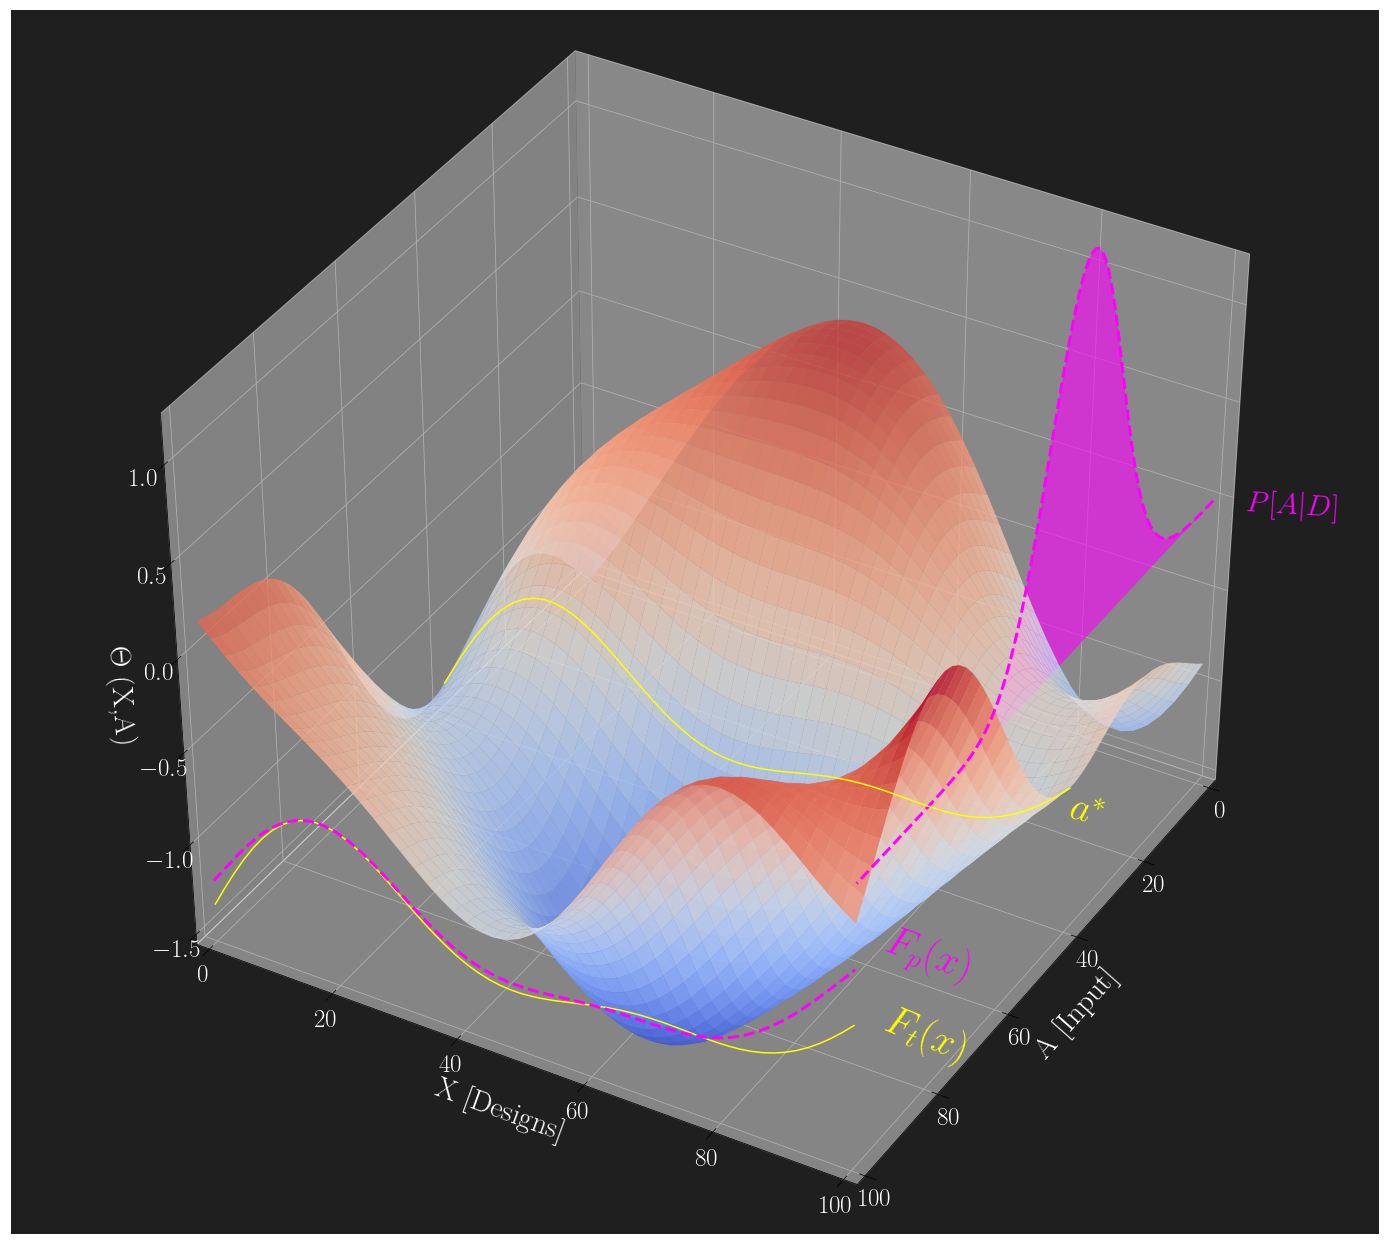
\includegraphics[width=7.0cm]{INTRO_IMAGE.png}\\
	\end{tabular}
\end{figure}
\end{frame}

\begin{frame}{Introduction}

Approximating the simulation runs, $\Theta (x,a)$, with $\mu (x,a)$.

\begin{figure}
	\centering
	\begin{tabular}{cc}
		Sample $\{(x,a)\}$ & Collect data\\
		Update \textcolor{green}{$\mu (x,a)$}& Update \textcolor{magenta}{$\mathbb{P}[A|D]$}\\
		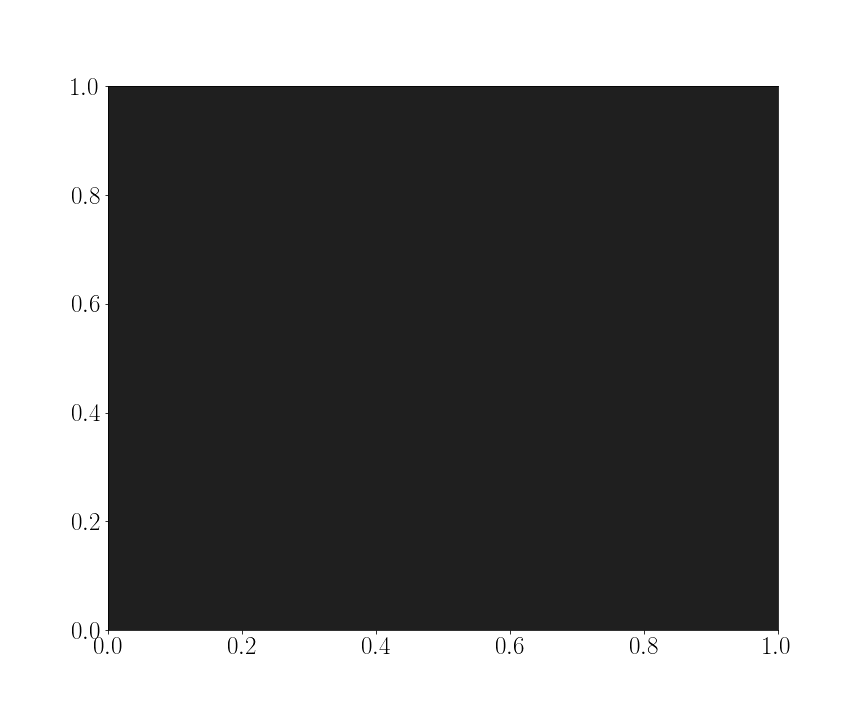
\includegraphics[width=5.5cm]{FILLING.png}&
		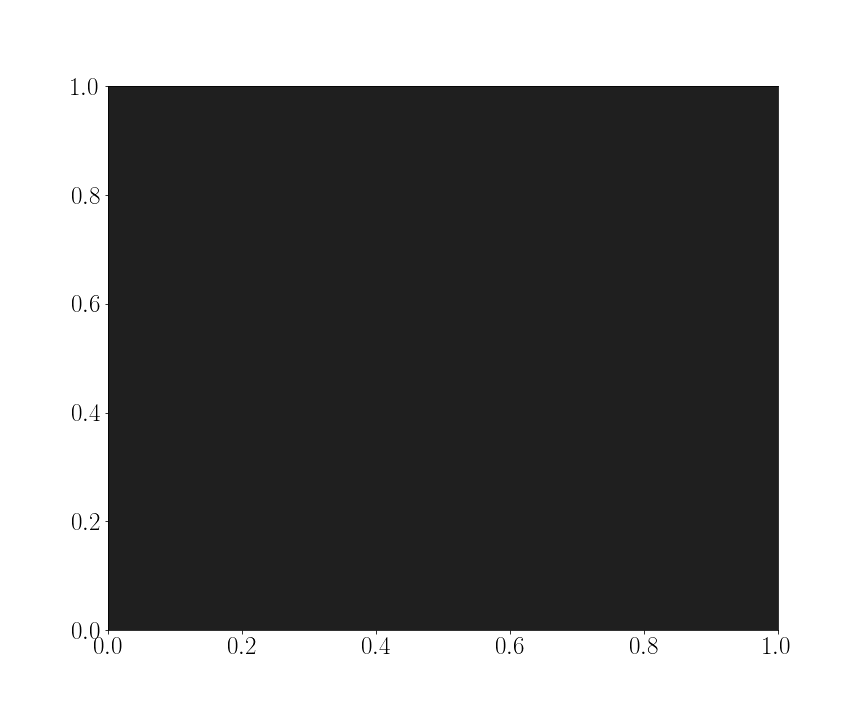
\includegraphics[width=5.5cm]{FILLING.png}\\
	\end{tabular}

$$ \hat{F}(x) = \int_{A} \textcolor{green}{\mu (x,a)} \textcolor{magenta}{\mathbb{P}[a|D]}da$$
\end{figure}
\end{frame}

\begin{frame}{Motivation}
\begin{itemize}
\item Goal: Minimise the difference between the maximum of the expected and true performance\\
\end{itemize}

	Constraint:
\begin{itemize}
	\item Fixed budget N.
\end{itemize}
\vspace{5mm}
Standard Approach:\\
Decide how to split N, then first collect more input distribution data, spend remaining budget on simulations.\\
\vspace{5mm}
Proposed Approach:\\
Sequentially allocate budget to either input data collection and update \textcolor{magenta}{$\mathbb{P}[a|D]$}, or run more simulations and update \textcolor{green}{$\mu(x,a)$}, depending on what seems to have largest benefit


\end{frame}




\section{Introduction to Bayesian Optimisation}


\section{Problem Formulation}
\begin{frame}{Gaussian Process Approximation}
Consider the possible designs $x \in X$, an unknown input value $a \in A$, and a function $\theta$: $X \times A \rightarrow \mathbb{R}$. 
 $$f(x,a) = \theta(x,a) +\epsilon$$
  where $\epsilon \sim N(0,\sigma^{2}_{\epsilon})$
  
  \begin{figure}
  	\centering
  	\begin{tabular}{c}
  		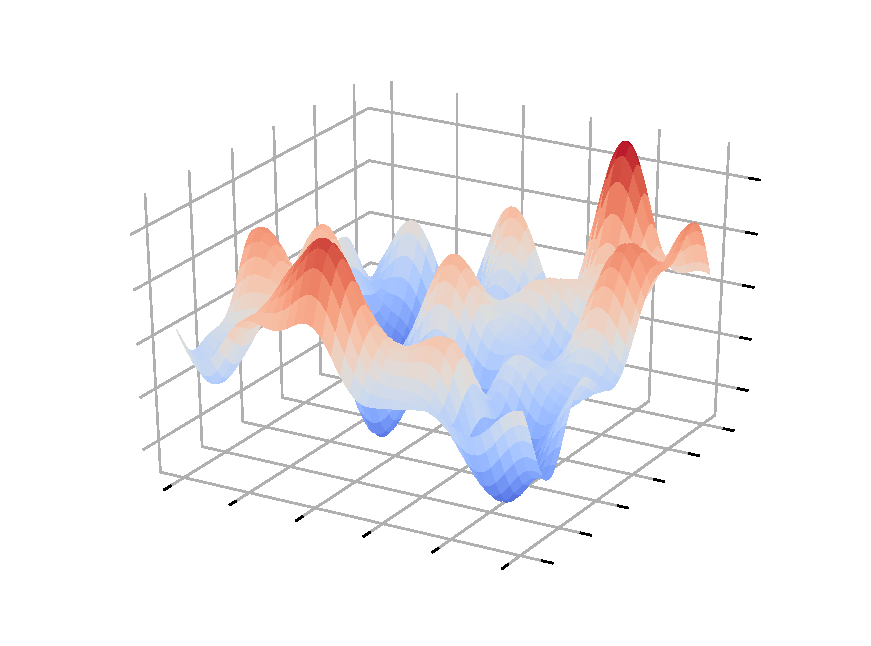
\includegraphics[width=4cm]{Presentation_plot_12.eps}\\
  	\end{tabular}
  \end{figure}
  Modelled by the mean \small{$\mu^{n}(x,a)$} \normalsize{and covariance} \small{$k^n((\mathbf{x},\mathbf{a});(\mathbf{x}',\mathbf{a}'))$} \normalsize{of a Gaussian process}.
  
\end{frame}



\begin{frame}{Problem Formulation: Expected Performance}

Identify the design $\mathbf{x}$ that maximises the expected performance:
$$\hat{F}(x) = \mathbb{E}_{\mathbb{P}[a|D^{m}]}[\mu(\mathbf{x},\mathbf{a})] = \int_{A}\textcolor{green}{\mu^{n}(x,a)}\textcolor{magenta}{\mathbb{P}[a|D^{m}]}da$$

\textcolor{green}{Data collection from simulation runs:}\\~\\
$R^{n} =\{(x, a, y)^{i}	|i = 1, . . . ,n\}$\\~\\

\textcolor{magenta}{Data collection from input sources:} \\~\\
$D^{m} = \{(j	,d)^{i}|i = 1, . . . ,m\}$; $d$ is an observation from the input $j \in \{1, . . . , I \}$


\end{frame}

\begin{frame}{Problem Formulation: Quality of Sampling}

The Opportunity Cost (OC): Difference in true performance between the design with the highest predicted value and the true best design

\begin{align*}
OC = \max_{x}F(x)-F(x_{r})
\end{align*}
where $F(x) = \theta(x,a^{*})$ and $\mathbf{x}_{r} = \textrm{arg}\max_{\mathbf{x}}\hat{F}(\mathbf{x})$

\begin{figure}
	\begin{center}
		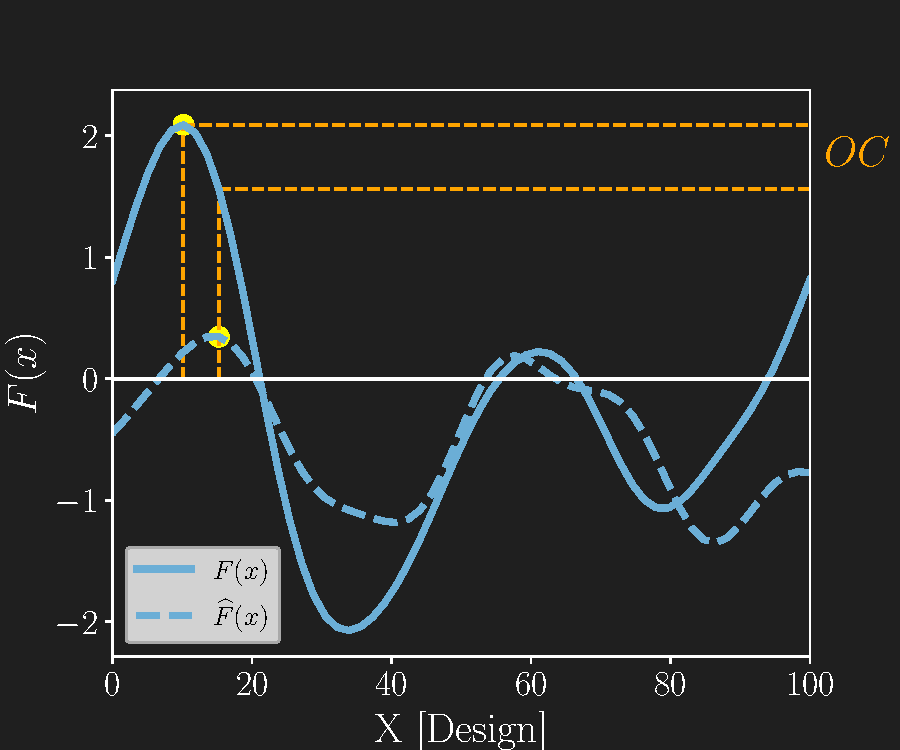
\includegraphics[width=6cm]{PROB_2.pdf}
	\end{center}
\end{figure}

\end{frame}


\begin{frame}[fragile,t]{Algorithm: Knowledge Gradient for Input Uncertainty}
[Pearce and Branke, (2017)]

\begin{columns}
	\begin{column}{0.6\textwidth}
		\begin{itemize}
			\item From current $\max_{\mathbf{x} \in X}\{\widehat{F}^n(\mathbf{x})\}$
			\vspace{5mm}
			\item Given a sample $(\mathbf{x},\mathbf{a})^{n+1}$
			\vspace{5mm}
			\item Update posterior $\mu^{n}(x,a)$
			\vspace{5mm}
			\item Update to $\max_{\mathbf{x} \in X}\{\widehat{F}^{n+1}(\mathbf{x})\}$
		\end{itemize}
	\end{column}

	\begin{column}{0.5\textwidth}  %%<--- here
		\begin{figure}
			\centering
			\begin{tabular}{c}
				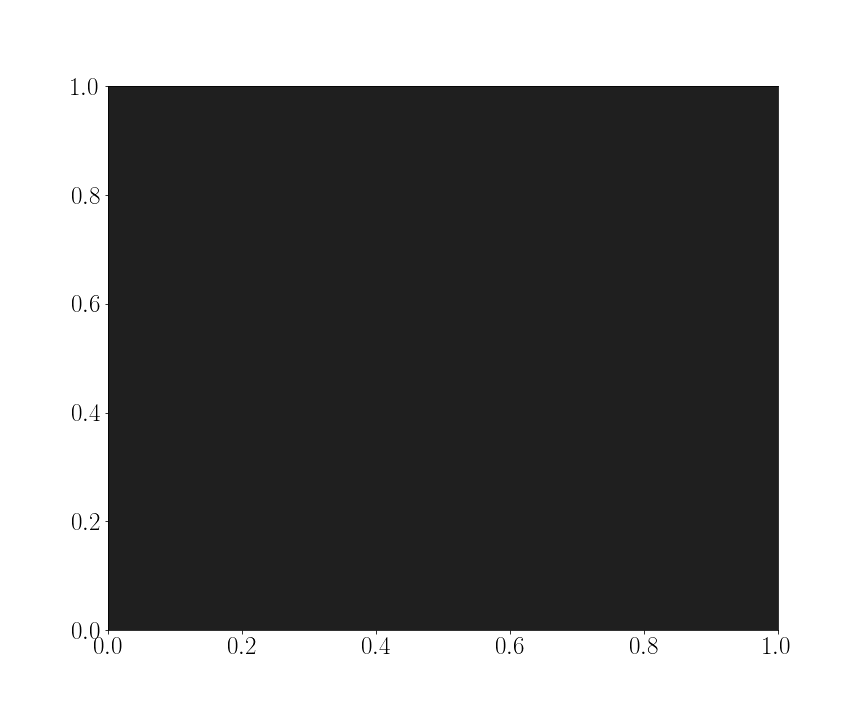
\includegraphics[width=5.5cm]{FILLING.png}\\
				$\widehat{F}(x) = \int_{A} \textcolor{green}{\mu^{n} (x,a)} \mathbb{P}[a|D]da$\\
			\end{tabular}
		\end{figure}
	\end{column}
\end{columns}

\end{frame}

\begin{frame}{Algorithm: Knowledge Gradient for Input Uncertainty}
[Pearce and Branke, (2017)]

Given a discretised set X, evaluate sample $(\mathbf{x},\mathbf{a})^{n+1}$ such maximises,

$$KG_{R}(\mathbf{x},\mathbf{a}) = \mathbb{E}[\max_{\mathbf{x}'' \in X}\{\hat{F}^{n+1}(\mathbf{x}'')\}|(\mathbf{x},\mathbf{a})^{n+1}]-\max_{\mathbf{x}'\in X}\{\hat{F}^n(\mathbf{x}')\}$$
\end{frame}



\section{Input Parameter Update}
\begin{frame}{Algorithm: Input Uncertainty Reduction}

\begin{figure}
	\centering
	\begin{tabular}{c}
		Collect data\\
		Update \textcolor{magenta}{$\mathbb{P}[A|D]$}\\
		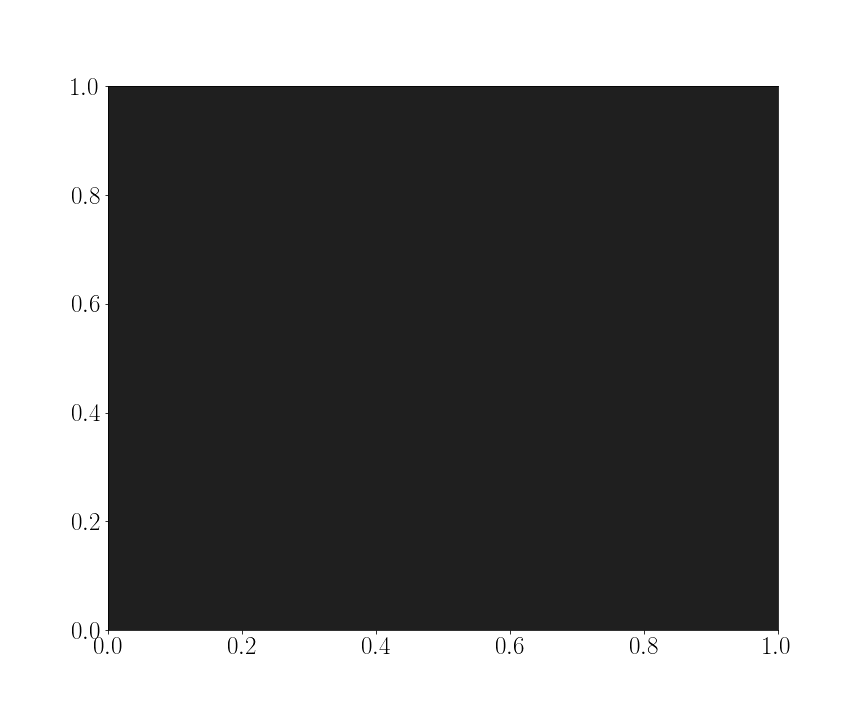
\includegraphics[width=5.5cm]{FILLING.png}\\
	\end{tabular}
	
	$$ \hat{F}(x) = \int_{A} \mu^{n} (x,a) \textcolor{magenta}{\mathbb{P}[a|D]}da$$
\end{figure}

\end{frame}

\section{Input Parameter Update}
\begin{frame}{Algorithm: Input Uncertainty Reduction}

Given the true value $a_{j}^{*}$ of an input $j \in \{1, . . . , I\}$,

$$\widehat{OC} = \max_{x}\mu(\mathbf{x},a^{*}) - \mu(\mathbf{x}_{r},a^{*})$$

Thus, the expected overall loss across aosterior ll the input distribution.

$$Loss(D^{m}) = \EX_{\mathbb{P}[a|D^{m}]}[\max_{x}\mu(\mathbf{x},a) - \mu(\mathbf{x}_{r}(D^{m}),a))]$$

$D^{m} = \{(j	,d)^{i}|i = 1, . . . ,m\}$; $d$ is an observation from the input $j \in \{1, . . . , I \}$
\end{frame}


\begin{frame}{Algorithm: Input Uncertainty Reduction}
Given a sample $(j,d)^{m+1}$ from an input source,
\begin{equation*}
Loss^{j}(D^{m+1}) = \EX_{\mathbb{P}[d_{m+1}|D^{m}]}[ \EX_{\mathbb{P}[a|D^{m+1}]}[\max_{x}\mu(\mathbf{x},a) - \mu(\mathbf{x}_{r}(D^{m+1}),a)]]
\end{equation*}

Finally, the expected difference reduction is as follows:


\begin{align*}
\begin{split}
KG_{I}^{j} &= Loss^{m}(D^{m}) - Loss^{j}(D^{m+1})\\
&=\EX_{\mathbb{P}[d_{m+1}|D^{m}]}[\EX_{\osterior mathbb{P}[a|D^{m+1}]}[ \mu(\mathbf{x}_{r}(D^{m+1}),a)- \mu(\mathbf{x}_{r}(D^{m}),a)]]
\end{split}
\end{align*}
\end{frame}

\begin{frame}{Algorithm: Decision Rule (DR)}



The measure that gives greater improvement, either $KG_{R}$ or $KG^{j}_{I}$
for any of the inputs $j \in \{1,\dots,n\}$, will state whether if we sample
$(x,a)^{n+1}$, or $(j, d)^{m+1}$.

\begin{figure}
	\centering
	\begin{tabular}{cc}
		Sample $\textcolor{green}{\{(x,a)\}}$ & Sample $\textcolor{magenta}{(j, d)^{m+1}}$\\
		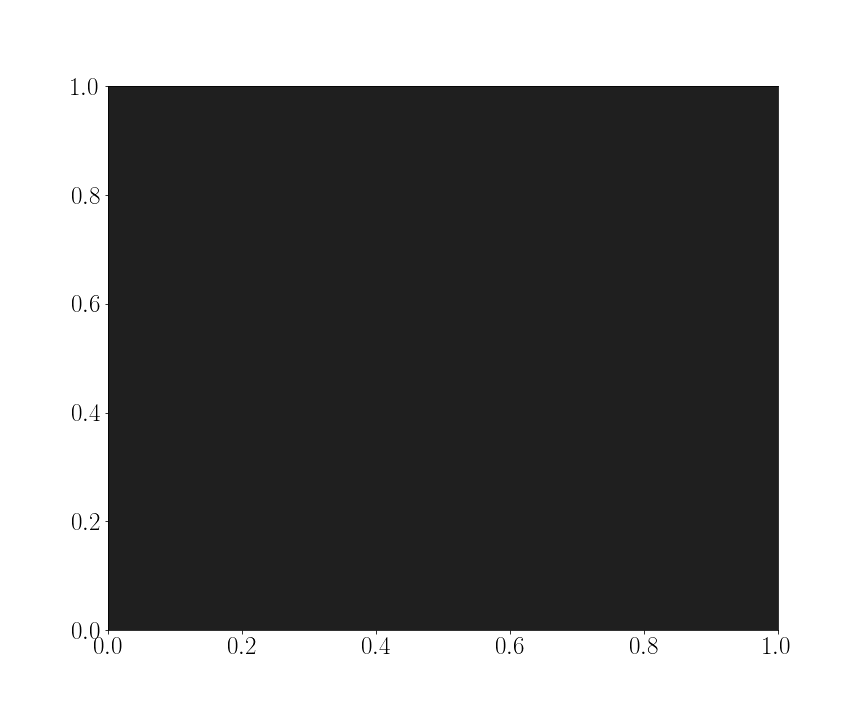
\includegraphics[width=5.5cm]{FILLING.png}&
		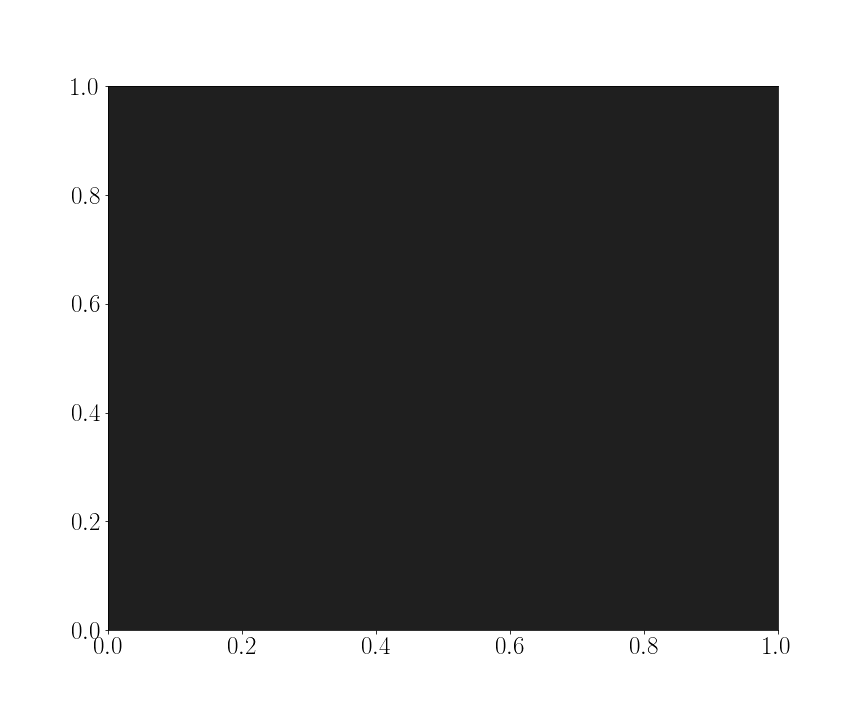
\includegraphics[width=5.5cm]{FILLING.png}\\
	\end{tabular}
	osterior 
	$$ \widehat{F}(x) = \int_{A} \textcolor{green}{\mu (x,a)^{n}} \textcolor{magenta}{\mathbb{P}[a|D]}da$$
\end{figure}


\end{frame}

\begin{frame}{Numerical Experiments: Test Problem}
Test Function (1 Design, 1 Input): 
\begin{itemize}
	\item Gaussian process with a squared exponential kernel.
	\item Hyperparameters: $l_{XA} = 10$, $\sigma_{0}^{2}=1$ $\sigma_{\epsilon}^{2}=0.1$
	\item Design $x \in X = [0, 100]$, and an input $a \in A = [0, 100]$.
\end{itemize}
Input parameter:
\begin{itemize}osterior 
	\item Data $d^{j} \sim N(a_{j}^{*},\sigma_{j}^{2})$ for $j=1$
	\item We use a Normal Likelihood and Uniform prior for inference $\mathbb{P}[A|D^{m}]$ 
\end{itemize}
\end{frame}
\begin{frame}{Numerical Experiments: Test Problem}

Test Function (1 Design, 2 Inputs): 
\begin{itemize}
	\item Gaussian process with a squared exponential kernel.
	\item Hyperparameters: $l_{XA} = 10$, $\sigma_{0}^{2}=1$ $\sigma_{\epsilon}^{2}=0.1$
	\item Design $x \in X = [0, 100]$, and an input $a^{1},a^{2} \in A = [0, 100]$.
\end{itemize}
Input parameter:
\begin{itemize}
	\item Data $d^{j} \sim N(a_{j}^{*},\sigma_{j}^{2})$ for $j=1,2$
	\item We use a Normal Likelihood and Uniform prior for inference $\mathbb{P}[A|D^{m}]$ 
\end{itemize}
\end{frame}osterior 

\begin{frame}{Numerical Experiments: Benchmark Method}

Given a total budget of $N$ and ratio $p$ from total budget.\\~\\

\begin{itemize}
	\item Stage 1: Sample $Np$ and update the input distribution $P[a_{j}|D^{m}]$. Samples are uniformly distributed for multiple inputs.
	\item Stage 2: Update $\mu ^{n}(x,a)$ with $N(1-p)$ samples allocated using $KG_{R}(x,a)$.
\end{itemize}
\end{frame}

\begin{frame}{Numerical Experiments: Results}
\begin{figure}[H]
	\centering
	\begin{tabular}{cc}
		1 Input  &2 Inputs\\
		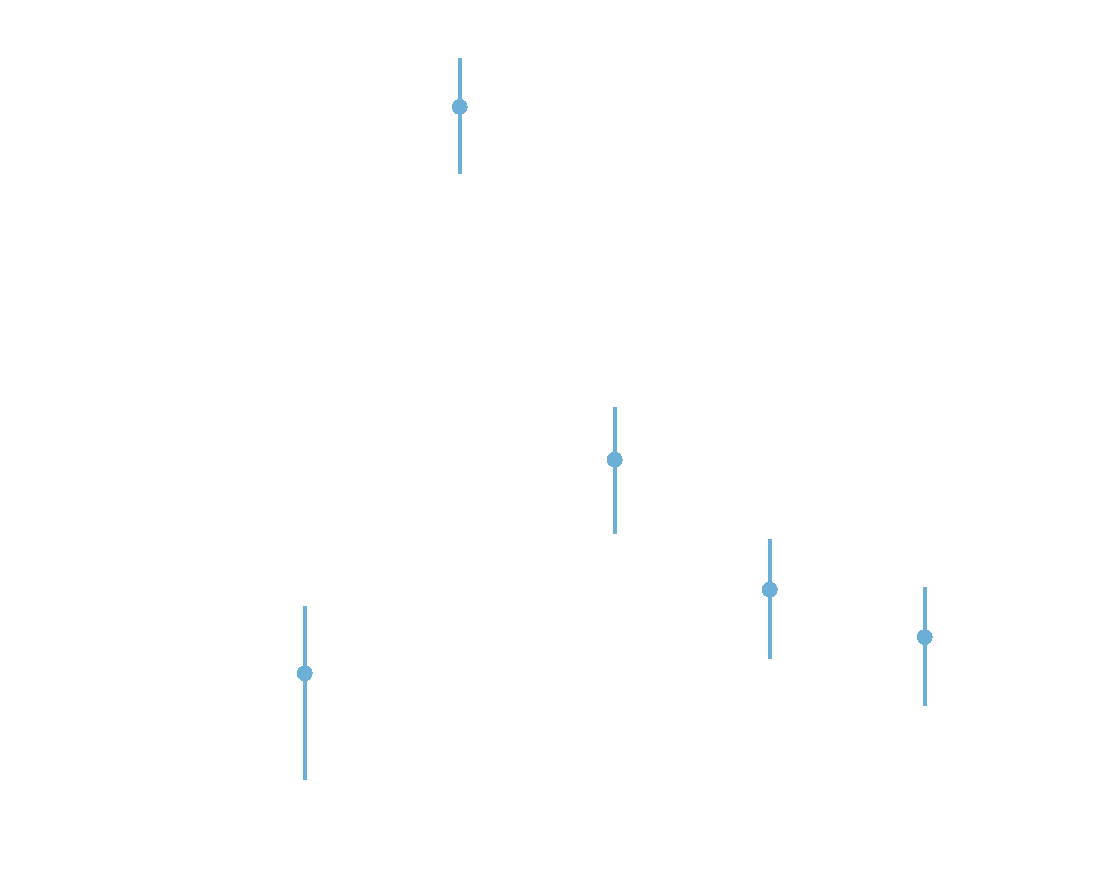
\includegraphics[width=5.2cm]{comparisons_1D.pdf} &
		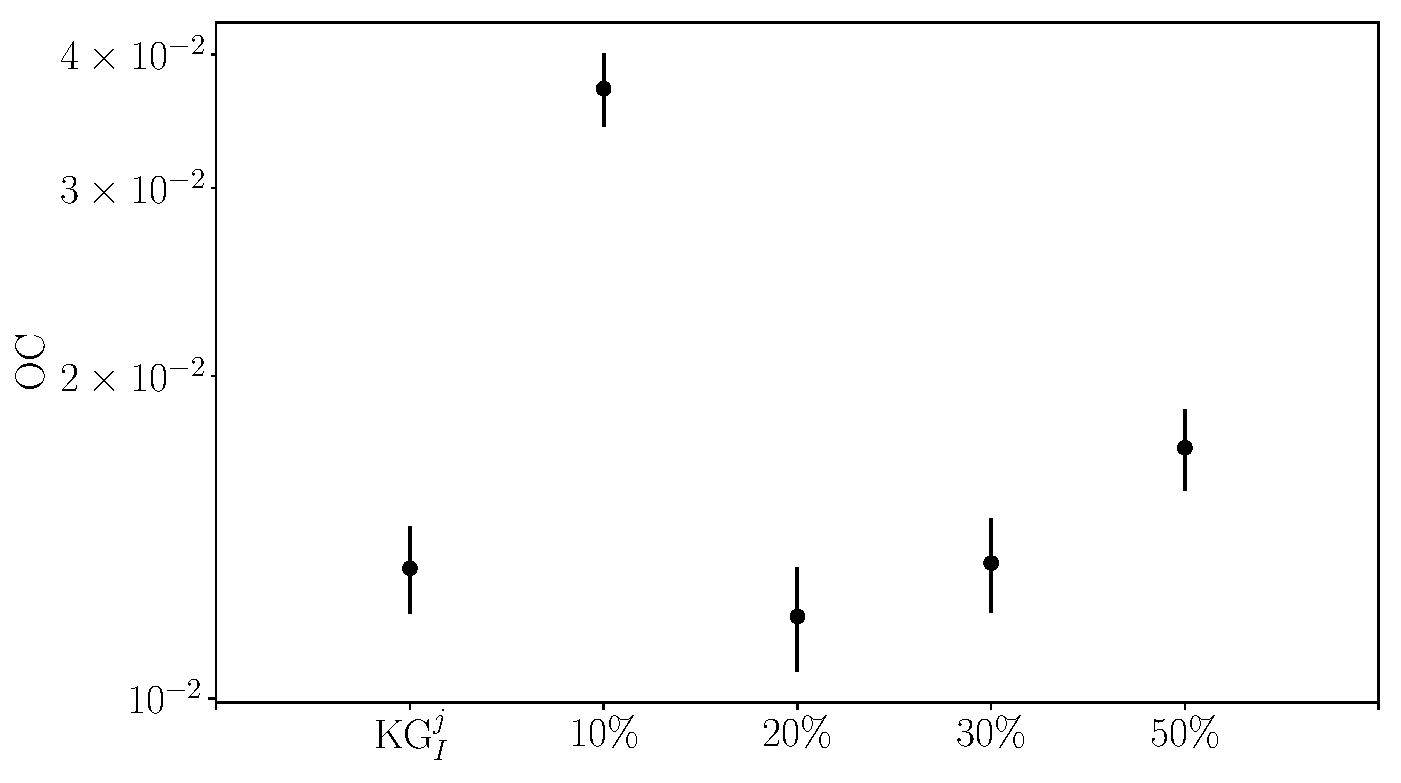
\includegraphics[width=5.5cm]{comparisons_2D.pdf}\\
		
	\end{tabular}
\end{figure}

\end{frame}osterior 

\section{Numerical Experiments}
\begin{frame}{Numerical Experiments}
	\begin{figure}[H]
		\centering
		\begin{tabular}{cc}
			p=1 \% &p=5 \% \\
			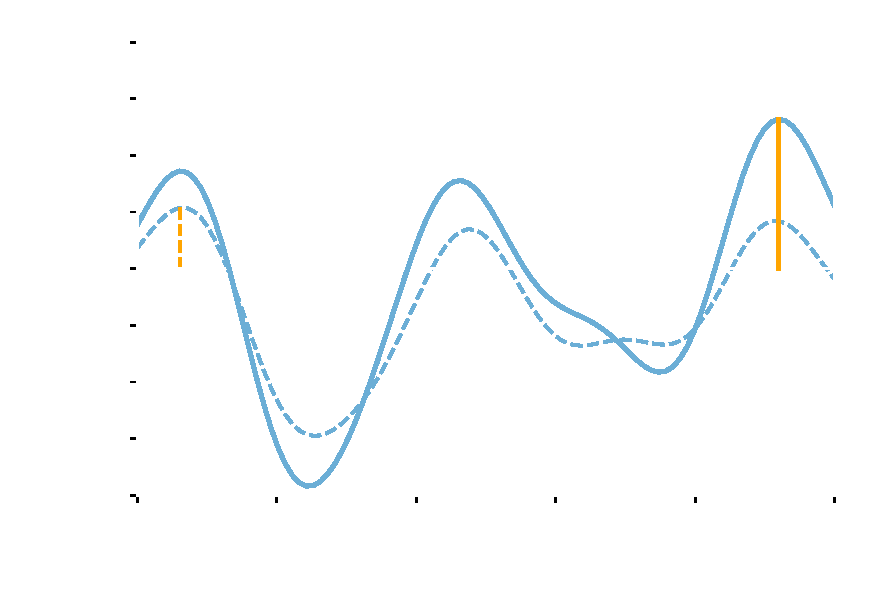
\includegraphics[width=5cm]{c_F_a_1.eps}&
			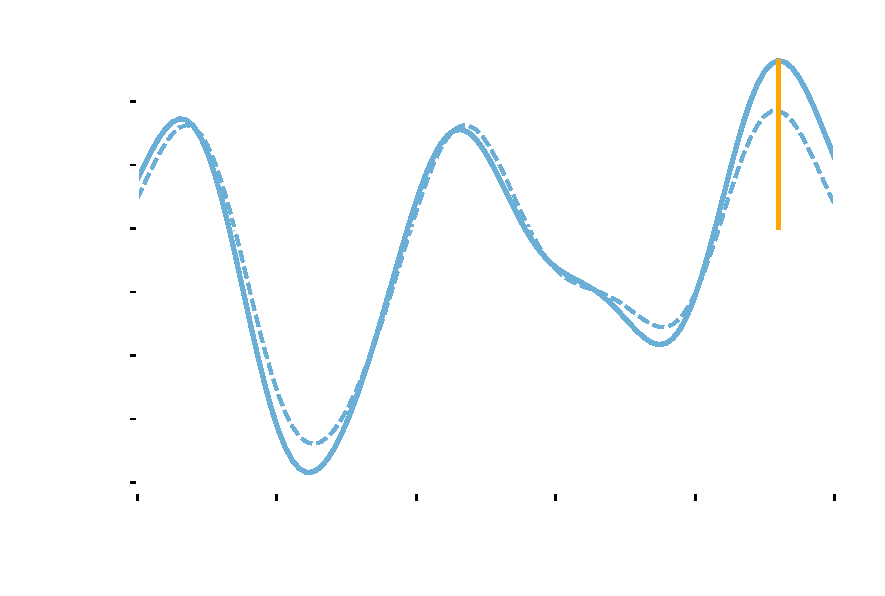
\includegraphics[width=5cm]{c_F_a_5.eps}\\
			
			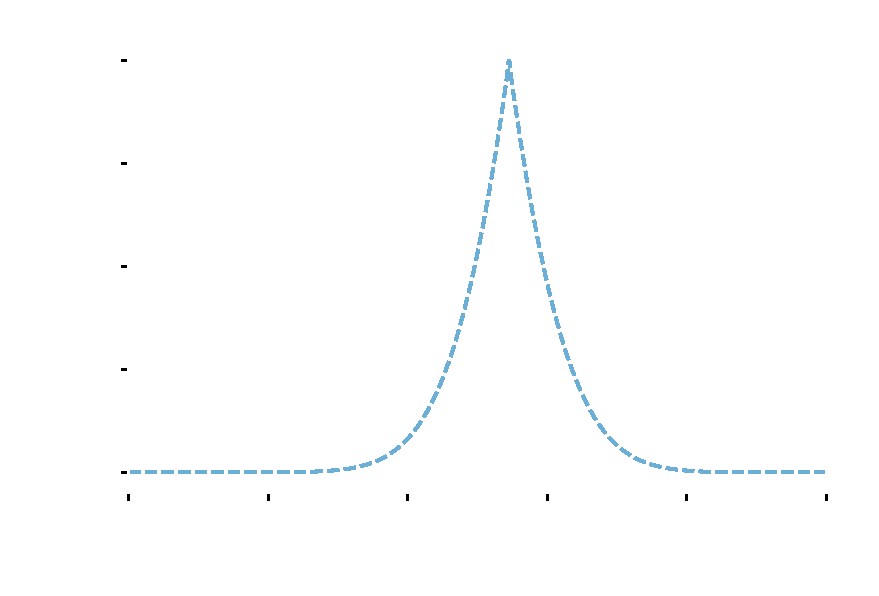
\includegraphics[width=5cm]{c_P_x_1.eps}&
			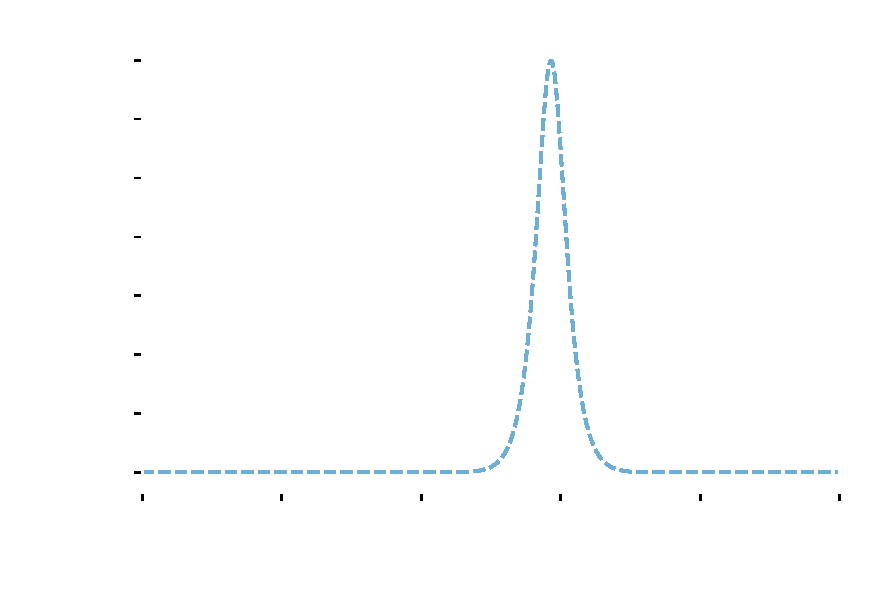
\includegraphics[width=5cm]{c_P_x_5.eps}\\

			
		\end{tabular}
	\end{figure}
\end{frame}

\begin{frame}{Numerical Experiments}
	\begin{figure}[H]
		\centering
		\begin{tabular}{cc}
			
			p=10 \%& p=50 \% \\
			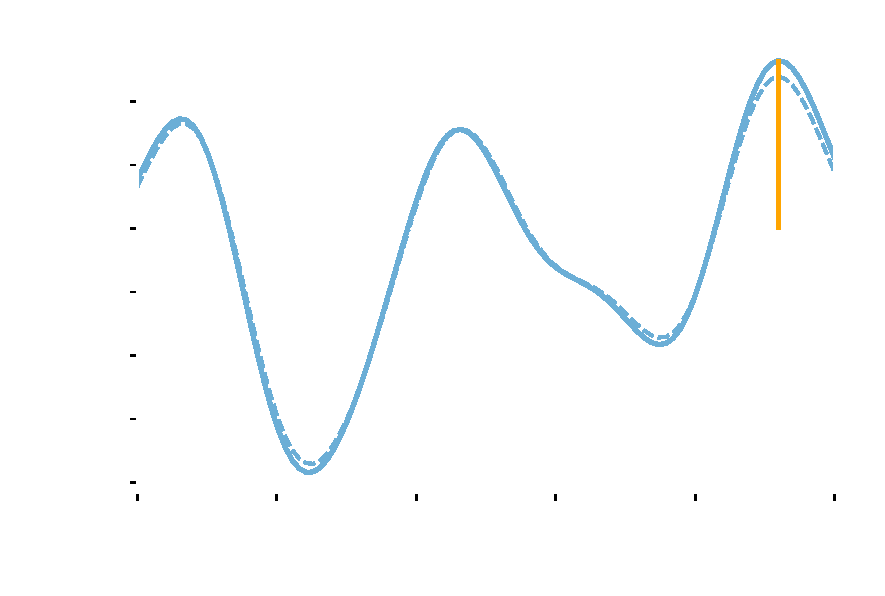
\includegraphics[width=5cm]{c_F_a_10.eps}&
			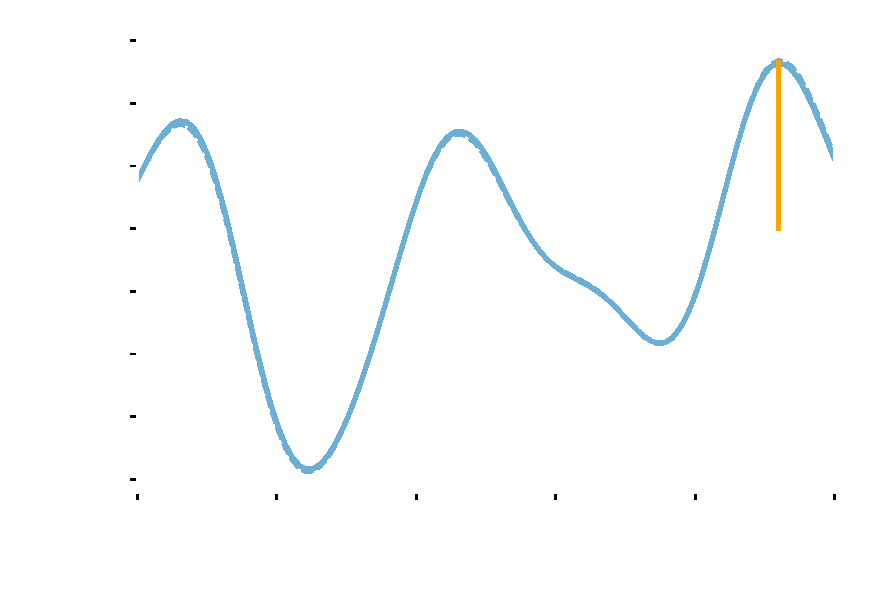
\includegraphics[width=5cm]{c_F_a_50.eps}\\
			
			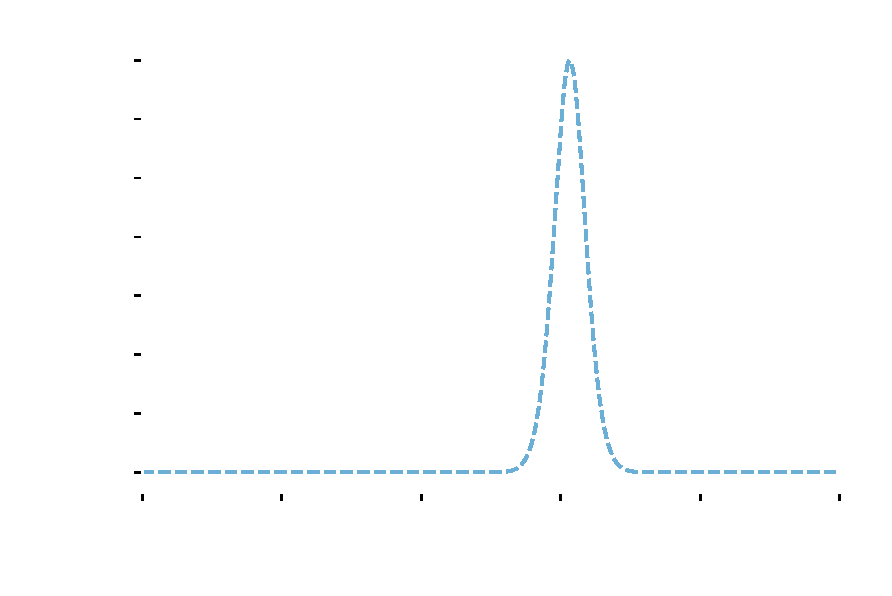
\includegraphics[width=5cm]{c_P_x_10.eps}&
			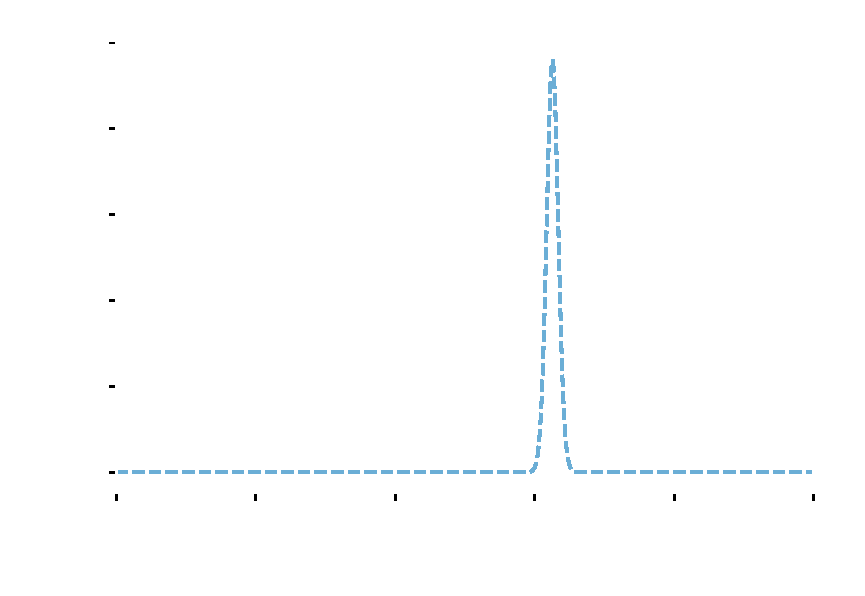
\includegraphics[width=5cm]{c_P_x_50.eps}\\
			
		\end{tabular}
	\end{figure}
\end{frame}



\section{Conclusions}
\begin{frame}{Conclusions}
	\begin{itemize}
		\item  The algorithm is capable of balancing between running additional simulations and reducing the input uncertainty.\\~\\
		\item Including $KG_{I}^{j}$ to allocate samples presents a similar performance respect of choosing an "adequate" fixed proportion in a 2-stage sampling.\\~\\
		\item The developed metric does not depend of parameters set by the user.\\~\\
	\end{itemize}
\end{frame}


\end{document}